\boldmath
\chapter{La fonction zêta de Riemann}	
\unboldmath
	Au \siecle{14} siècle l'évêque de Lisieux Nicole Oresme\personne[économiste, mathématicien, physicien, astronome, philisophe, psychologue, musicologue, théologien et traducteur français]{Nicole}{Oresme}{1320}{1382} savait déjà que la série harmonique~$\sum_{n\geq 1} 1/n$ est une série divergente. En 1644, le mathématicien italien Pietro Mengoli (1626--1686) s'intéresse à la série de terme général~$1/n^2$ et se alors pose la question de la limite de cette série. 
		
	Ce problème, connu sous le nom de problème de Mengoli (ou problème de Bâle), reste ouvert jusqu'en 1735, où le mathématicien suisse Leonhard Euler (1707--1783) conjecture que la série admet pour limite~$\pi^2/6$ ; mais ce n'est qu'en 1748 qu'il en obtient une démonstration rigoureuse.
		
	Euler ne s'arrête pas là, et démontre une formule plus générale : pour tout entier~$k$ supérieur ou égal à~$1$ il énonce que
	\[
		\sum_{n=1}^{+\infty} \frac{1}{n^{2k}} =
			-\frac{B_{2k} (2i\pi)^{2k}}{2(2k)!}\cdot
	\]
	Où~$B_n$ est le~$n$-ième nombre de Bernoulli\personne[mathématicien et physicien suisse]{Jacques}{Bernoulli}{1654}{1705} (voir paragraphe~\ref{subsection:nombrBernoulli}). Euler introduit ainsi la fonction zêta ; pour tout réel~$x$ strictement supérieur à~$1$ il pose
	\[
		\zeta(x) = \sum_{n=1}^{+\infty} \frac{1}{n^x}\cdot
	\]
	Grâce à la méthode du crible d'Ératosthène il démontre la formule suivante, connue sous le nom de produit eulérien, formule que nous redémontrerons dans le cas complexe :
	\[
		\zeta(x) = \prod_{p\in\Pre} \left( 1-\frac{1}{p^x} \right)^{-1}.
	\]
	Cette formule est alors la première à faire le lien entre l'analyse (avec la fonction zêta) et les nombres premiers.
	
	C'est en 1859 dans son article de 8 pages, devenu aujourd'hui incontournable : \textit{Über die Anzahl der Primzahlen unter einer gegebenen Grö\ss{}e} \footnote{Sur le nombre de nombres premiers inférieurs à une taille donnée.} (cf.~\cite{ArticRiemann}), que Riemann a l'idée d'étendre la fonction zêta aux nombres complexes de partie réelle strictement supérieure à~$1$ puis au plan complexe privé de~$1$. Riemann y démontre aussi l'équation fonctionnelle de zêta (cf. théorème~\ref{thm:EquaFonctZeta}) et y formule la conjecture, connue sous le nom d'\emph{hypothèse de Riemann}, qui sera l'objet de notre troisième partie.
	
	Dans cette partie nous allons introduire la fonction zêta, communément appelée \emph{fonction zêta de Riemann} depuis les travaux de ce dernier sur cette fonction. Nous verrons ici le prolongement de zêta à l'ensemble des nombres complexes différents de~$1$ et les premières propriétés de cette application.
\section{Quelques mots sur les séries de Dirichlet}
		\begin{defi}
			On appelle série de Dirichlet toute application~$F$ définie sur une partie de~$\mathbb{C}$ et à valeur complexe, de la forme :
			\[
				F(s) = \sum_{n=1}^{+\infty} \frac{a_n}{n^s},
			\]
			où~$s$ est une variable complexe et où~$\suite*{a}$ est une suite de nombres complexes.
		\end{defi}
		\begin{prop}
			Soit~$F(s)=\sum_{n\geq 1} \frac{a_n}{n^s}$ une série de Dirichlet et~$s_0$ un nombre complexe tel que la série~$F(s_0)$ soit convergente, alors pour tout réel~$C$ positif ou nul~$F$ est absolument convergente sur l'ensemble
			\[
				E_{C,s_0} = \{s\in\mathbb{C},\Re(s)\geq\Re(s_0),\abs{s-s_0}\leq C\,\Re(s-s_0)\}.
			\]
		\end{prop}
		\begin{dem}
			Pour tout réel~$M$ supérieur ou égal à~$1$,  on définit la fonction~$A_M$ donnée par~$A_M(x)=\sum_{M<n\leq x} a_n n^{-s_0}$. Par hypothèse sur~$s_0$, pour tout~$x$ dans~$\mathbb{R}$ on a~$A_M(x)$ tend vers~$0$ quand~$M$ tend vers l'infini ; aussi, il existe une application~$\epsilon :\mathbb{R} \rightarrow\mathbb{R}_+$ décroissante qui tend vers~$0$ en~$+\infty$ et telle que pour tout réel~$M$ supérieur ou égal à~$1$, on ait l'inégalité~$\abs{A_M(x)}\leq\epsilon(M)$. Soient maintenant~$s$ un nombre complexe et~$M,N$ deux entiers vérifiant~$1\leq M<N$, on peut utiliser la formule sommatoire d'Abel (proposition~\ref{prop:SomAbel}) pour obtenir  le calcul :
			\begin{equation}\label{eq:DirichPropDem}
				\sum_{M<n\leq N} \frac{a_n}{n^s} = \sum_{M<\leq N} \frac{a_n}{n^{s_0}n^{s-s_0}}
				= \frac{A_M(N)}{N^{s-s_0}} + (s-s_0) \int_{M}^{N} \frac{A_M(x)}{x^{s-s_0}} \,\mathrm{d}x.
			\end{equation}
			On pose ensuite~$\sigma_0=\Re(s_0)$ et~$\sigma=\Re(s)$, et on majore l'intégrale précédente en valeur absolue grâce à la décroissance de la fonction~$\epsilon$ :
			\[
				\abs{\int_M^N \frac{A_M(x)}{x^{s-s_0}}\mathrm{d}x} \leq \epsilon(M) \frac{M{-(\sigma-\sigma_0)}-N^{-(\sigma-\sigma_0)}}{\sigma-\sigma_0}\cdot
			\]
			On suppose ensuite~$s$ dans le secteur angulaire~$E_{C,s_0}$ que l'on a représenté dans la figure~\ref{fig:secteurAng}.
			\begin{figure}[h]
				\begin{multicols}{2}
					\begin{center}
						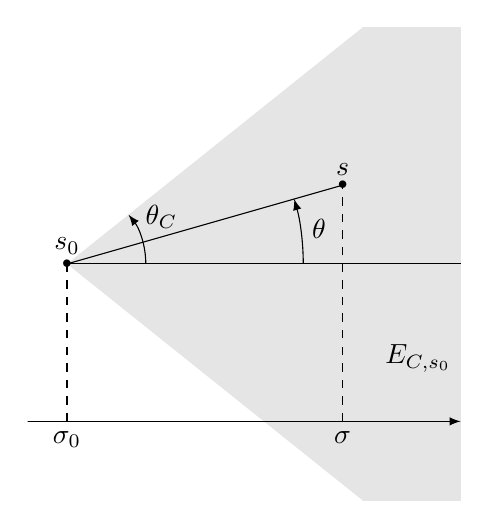
\begin{tikzpicture}
							%Clip
							\clip (-0.5,-1) rectangle (5,5) ; 
							%Secteur
							\fill [color=gray!20] (0,2) -- ++ (5,-4) -- ++ (0,8) -- cycle ;
							%Axes
							\draw [->,>=latex]	(-1,0)	-- (5,0) ;
							%Droites
							\draw [dashed]		(0,0)	-- (0,2)	;
							\draw [dashed]		(3.5,0)	-- (3.5,3)	;
							\draw [thin]		(0,2)	-- (5,2)	;
							\draw [thin]		(0,2)	-- (3.5,3)	;
							%Points
							\path [below]		(0,0)		node 				{$\sigma_0$}	;
							\path [below]		(3.5,0)		node				{$\sigma$}		;
							\path 				(0,2)		node [scale=0.7]	{$\bullet$}		;
							\path [above]		(0,2)		node 				{$s_0$}			;
							\path 				(3.5,3)		node [scale=0.7]	{$\bullet$}		;
							\path [above]		(3.5,3)		node 				{$s$}			;
							\path 				(3.2,2.45)	node				{$\theta$}		;
							\path				(1.2,2.6)	node				{$\theta_C$}	;
							\path [left]		(5,0.8)		node				{$E_{C,s_0}$}	;
							%Arc
							\draw [->,>=latex]	(1,2) arc (0:38.660:1)	;
							\draw [->,>=latex]	(3,2) arc (0:15.945:3)	;
						\end{tikzpicture}
					\end{center}
					\columnbreak
					
					Où, avec les notations introduites dans le dessin, on a~$C=1/\cos(\theta_C)$.
					
					En effet, on a clairement (pour le cas~$\theta\geq 0$) l'inégalité~$\theta\leq\theta_C\leq\pi/2$ ; puis, par décroissance du cosinus sur~$[0,\pi/2]$, il s'en suit l'inégalité~$\cos(\theta)\leq\cos(\theta_C)$. Le cas où~$\theta$ est négatif se traite de la même façon.
					
					Comme de plus on a, par construction, l'identité~$\sigma-\sigma_0 = \abs{s-s_0}\cos(\theta)$, il s'en suit~$\sigma-\sigma_0 \leq \abs{s-s_0}\cos(\theta_C)$.
				\end{multicols}
				\caption{Illustration du secteur angulaire~$E_{C,s_0}$.}
				\label{fig:secteurAng}
			\end{figure}
			Comme~$s$ vérifie les inégalités~$\sigma-\sigma_0\geq 0$ et~$\sigma-\sigma_0\leq C\abs{s-s_0}$, l'équation~\eqref{eq:DirichPropDem} nous fournit la majoration~$\abs{\sum_{m<n\leq N} a_n n^{-s}} \leq \epsilon(M)(1+C)$, or le terme de droite tend vers~$0$ quand~$M$ tend vers l'infini. Cela suffit à démontrer la convergence uniforme de la série dans le secteur~$E_{C,s_0}$.
		\end{dem}
		\begin{coro}
			Toute série de Dirichlet~$F(s)=\sum_{n\geq 1} \frac{a_n}{n^s}$ possède une abscisse~$\sigma_c$ (éventuellement infinie) appelée \emph{abscisse de convergence absolue} telle que pour tout~$s$ de partie réelle~$\sigma$ la série~$F(s)$ soit convergente pour~$\sigma>\sigma_C$ et divergente pour~$\sigma<\sigma_c$.
		\end{coro}
		\begin{dem}
			Il suffit de poser~$\sigma_c=\inf\{\sigma\in\mathbb{R},F(\sigma)\text{ converge}\}$, puis d'observer que tout compact du demi-plan ouvert~$\Omega_{\sigma_c}$ est contenu dans un secteur de la forme~$E_{C,\sigma}$ avec pour~$\sigma>\sigma_c$ et~$C\geq 0$. Comme, d'après la proposition précédente, on sait que~$F$ converge dans tout ces~$E_{C,\sigma}$ , on obtient la convergence dans~$\Omega_{\sigma_c}$.
			
			Pour montrer que~$F(s)$ diverge pour~$\sigma<\sigma_c$ il suffit de raisonner par l'absurde et de monter qu'alors~$\sigma_c$ ne serait pas borne inférieure précédemment définie.
		\end{dem}
\section{Définition et première propriétés de la fonction zêta de Riemann}
	\subsection{Définition}
		\begin{defi}
			On définit pour tout nombre complexe~$s$ de partie réelle strictement supérieure à~$1$ la \emph{fonction zêta de Riemann}, notée~$\zeta$\nomenclature[Gf]{$\zeta$}{Fonction zêta de Riemann}, en posant :~$\zeta(s) = \sum_{n\geq 1} \frac{1}{n^s}$.
		\end{defi}
		\begin{rem}
			En d'autre termes, la fonction zêta de~Riemann est la série de Dirichlet associée à la suite constante égale à~$1$. On sait, d'après le critère de convergence des séries de Riemann, que cette série diverge en~$s=1$. Aussi son abscisse de convergence absolue est supérieure ou égale à~$1$ ; la proposition suivante nous montre qu'en fait cette abscisse est~$1$.
		\end{rem}
		\begin{prop}
			La fonction~$\zeta$ est définie et holomorphe sur~$\Omega_1$.
		\end{prop}
		\begin{dem}
			\demsection{$\zeta$ définie}
			Soient~$s=\sigma+it$ un nombre complexe de partie réelle strictement supérieure à~$1$ et~$n$ un nombre entier non nul, on a~$\abs{n^s}= \abs{e^{\sigma\log(n)}\cdot e^{i\,t\log(n)}}=n^\sigma$ donc la série de terme général~$\frac{1}{n^s}$ est absolument convergente par le critère de Riemann sur les séries numériques.
			
			\demsection{$\zeta$ holomorphe}
			On se place sur~$\overline{\Omega}_{1+\epsilon}$ pour~$\epsilon$ un réel strictement positif. On va montrer que la série définissant~$\zeta$ converge normalement sur~$\overline{\Omega}_{1+\epsilon}$. On a
			\[
				\norme{\frac{1}{n^s}}_{\infty,\overline{\Omega}_{1+\epsilon}} = \sup_{s\in\overline{\Omega}_{1+\epsilon}} \abs{\frac{1}{n^s}} = \frac{1}{n^{1+\epsilon}},
			\]
			où~$\frac{1}{n^{1+\epsilon}}$ est le terme général d'une série de Riemann convergente. Ce qui justifie la convergence normale. Ainsi,~$\zeta$ est holomorphe sur~$\overline{\Omega}_{1+\epsilon}$ pour tout~$\epsilon$ strictement positif. Donc~$\zeta$ est holomorphe sur~$\Omega_1$.
		\end{dem}
	\subsection{Lien avec les nombres premiers}
		On rappelle que~$p_1,p_2,\ldots,p_n,\ldots$ désigne la suite croissante des nombres premiers.
		\begin{prop}[produit eulérien]\label{prop:produitEulerien}
			Pour tout nombre complexe~$s$ de partie réelle strictement supérieur a~$1$, on à l'identité
			\[
				\zeta(s) = \prod_{n=1}^{+\infty} \left( 1 - \frac{1}{p_n^s}\right)^{-1}.
			\]
			De plus, la convergence du produit est normale sur tout compact de~$\Omega_1$.
		\end{prop}
		\begin{dem}
			\demsection{convergence du produit infini} 
			On pose~$s=\sigma+it$. Montrer que le produit converge absolument revient à montrer que le produit de terme général~$1-\frac{1}{p_n^s}$ converge strictement. Il suffit donc de montrer que la série de terme général~$\frac{1}{p_n^s}$ converge absolument (théorème~\ref{thm:ConvAbsoSerie->Prod}).
			
			Pour tout entier~$n$, on a~$\abs{p_n^s} = p_n^\sigma$ ; puis, comme l'ensemble des nombres premiers est inclus dans l'ensemble des entiers naturels, on a l'inégalité~$\sum_{n=1}^\infty \frac{1}{p_n^\sigma} \leq \sum_{n=1}^\infty \frac{1}{n^\sigma}$. Enfin la somme à droite de l'inégalité est une série de Riemann convergente pour~$\sigma$ strictement plus grand que~$1$. Ce qui justifie la convergence absolue de la série et donc du produit infini défini plus haut.
			
			\demsection{Égalité}
			On cherche ici à appliquer la proposition~\ref{prop:sérieSuiteSousEnsemble} sur la série définissant la fonction~$\zeta$.
					
			Pour tout~$j\in\mathbb{N}^*$ et tout~$k\in\mathbb{N}$ on pose
			\begin{align*}
				A_{j,k}	&=\{n\in\mathbb{N}^*,n=p_1^{k_1} \cdots p_j^{k_j}, 
																k_1+\cdots  	+k_j=k\},\\
				A_j	   	&=\bigcup_{k=0}^{+\infty} A_{j,k}
						 = \{ n\in\mathbb{N}^*, n = p_1^{k_1}\cdots p_j^{k_j}, k_1,\cdots,k_j \in\mathbb{N} \}.
			\end{align*}
			Vérifions les conditions de la proposition~\ref{prop:sérieSuiteSousEnsemble} :
			\begin{itemize}
				\item la somme définissant~$\zeta$ est absolument convergente ;
				\item alors les~$A_j$ forment une suite croissante pour l'inclusion, car si un entier~$n$ est dans~$A_j$, il peut s'écrire~$n=p_1^{k_1}\cdots p_j^{k_j}$ mais aussi~$n = p_1^{k_1}\cdots p_j^{k_j} \cdot p_{j+1}^0$ et donc il appartient à~$A_{j+1}$ ;
				\item l'union des~$A_j$ est, bien entendu, incluse dans~$\mathbb{N}^*$ et, par le théorème fondamental de l'arithmétique, on a l'inclusion inverse. Ce qui justifie que~$\bigcup_{j=1}^\infty A_j = \mathbb{N}^*$.
			\end{itemize}
			Tout ceci nous permet d'appliquer la proposition, on a
			\[
				\zeta(s) 	= \sum_{n=1}^{+\infty}\frac{1}{n^s}
							= \lim_{j\rightarrow\infty} \sum_{n\in A_j} \frac{1}{n^s}\cdot
			\]
			De plus, si on fixe un entier non nul~$j$,  alors la famille~$\left(A_{j,k}\right)_{k\in\mathbb{N}}$ forme une partition de~$A_j$, en effet :
			\begin{itemize}
				\item tous les~$A_{j,k}$ sont non vides ($p_1^k\in A_{j,k}$) ;
				\item si~$k$ et~$k'$ sont deux entiers, et que~$n$ est dans~$A_{j,k}\cap A_{j,k'}$, alors l'unicité de la décomposition d'un entier non nul en facteurs premiers assure que~$k=k'$ ;
				\item par définition de~$A_j$, on a bien~$\bigcup_{k\in\mathbb{N}} A_{j,k} = A_j$.
			\end{itemize}
			On peut enfin calculer 
			\begin{align*}
				\sum_{n\in A_j} \frac{1}{n^s}
							& = \sum_{k\in\mathbb{N}}\sum_{n\in A_{j,k}} \frac{1}{n^s}
							  = \sum_{k\in\mathbb{N}}\sum_
							  		{\substack{(k_1,\ldots,k_j)\in\mathbb{N}^j\\
							  					k_1+\cdots+k_j = k}}
							  		\frac{1}{\left(
							  			p_1^{k_1}\cdots p_j^{k_j}
							  			\right)^s
							  		}\\
							& = \left(\sum_{k_1=0}^{+\infty}\frac{1}{p_1^{k_1 s}}\right)
								\cdots
								\left(\sum_{k_j=0}^{+\infty}\frac{1}{p_1^{k_j s}}\right)
							  = \left(\frac{1}{1-\frac{1}{p_1^s}}\right)
							  	\cdots
							  	\left(\frac{1}{1-\frac{1}{p_1^s}}\right).
			\end{align*}
			On passe maintenant à la limite selon~$j$ :
			\[
				\zeta(s) = \prod_{j=1}^{+\infty} \left( 1 - \frac{1}{p_j^s} \right)^{-1}.
			\]
			\demsection{Convergence normale sur les compacts de~$\Omega_1$}
			Si~$K$ est un compact de~$\Omega_1$ que l'on suppose inclut dans~$\overline{\Omega}_{1+\epsilon}$ pour~$\epsilon$ un réel strictement positif ; alors la norme infinie de~$s\rightarrow \frac{1}{p_n^s}$ sur~$K$ est inférieur à~$\frac{1}{p_n^{1+\epsilon}}$. Où la série de terme général~$\frac{1}{p_n^{1+\epsilon}}$ est inférieure à la série de terme général~$\frac{1}{n^{1+\epsilon}}$, qui est le terme général d'une série de Riemann convergente. D'où la convergence normale sur~$K$.
		\end{dem}
		\begin{rem}
			La démonstration de l'égalité~$\sum_{n\geq 1} 1/n^s = \prod_{p\in\Pre} (1-p^{-s})^{-1}$ ne requiert pas l'hypothèse~$\Re(s)>1$ si ce n'est pour la convergence de la série. En d'autre termes, on peut la considérer comme une égalité formelle sans sous soucier de la convergence. L'identité du produit eulérien nous fournit alors une autre démonstration de l'infinité des nombres premiers. En effet si, par l'absurde, il y avait un nombre fini de nombres premiers, le terme de droite dans l'égalité convergerait pour~$s=1$ ; or le terme de gauche, lui, devient une série de Riemann divergente : c'est impossible.
		\end{rem}
		\begin{coro}\label{coro:zero}
			La fonction~$\zeta$ ne s'annule pas sur~$\Omega_1$.
		\end{coro}
		\begin{dem}
			Ceci est clair, au vu de l'expression de~$\zeta$ sous forme de produit infini dans la proposition précédente. En effet, la convergence normale du produit nous fournit la convergence normale de la série de terme général~$1-p_n^{-s}$ et donc la convergence stricte du produit, grâce au théorème~\ref{thm:ConvAbsoSerie->Prod}.
		\end{dem}
	\boldmath
	\subsection{Prolongement sur~$\Omega_0$}
	\unboldmath
		\begin{prop}\label{prop:P5}
			La fonction~$\zeta$ se prolonge en une fonction méromorphe dans le demi-plan ouvert~$\Omega_0$. Elle admet un unique pôle en~$1$, de résidu~$+1$. Ainsi, pour tout~$s$ dans~$\Omega_0$ on a
			\[
				\zeta(s) = \frac{1}{s-1} + 1 + s\int_{1}^{+\infty} (\entier{u}-u)u^{-s-1}\,\mathrm{d}u.
			\]
		\end{prop}
		\begin{dem}
			Soit~$s=\sigma+it$, on cherche à montrer que~$\zeta-\frac{1}{s-1}$ admet un prolongement holomorphe sur~$\Omega_0$. Pour cela, on va appliquer la formule sommatoire d'Abel (proposition~\ref{prop:SomAbel}) où, avec les notations de la proposition, on prend~$x,y$ deux réels vérifiant~$0<y<1\leq x$ et~$A(u)=\sum_{1\leq n\leq u} 1 =\entier{u}$. On obtient 
			\begin{align*}
				&&\displaystyle\sum_{y<n\leq x} \dfrac{1}{n^s} 		& =  \dfrac{\entier{x}}{x^s}- 	\dfrac{\entier{y}}{y^s}-\displaystyle\int_y^x \entier{u}(-s)u^{-s-1}\,\mathrm{d}u,	\\
				\text{soit }&&
				\displaystyle\sum_{1\leq n\leq x} \dfrac{1}{n^s} 	& = \dfrac{\entier{x}}{x^s} -0+s\displaystyle\int_y^x \entier{u}u^{-s-1}\,\mathrm{d}u	
				\quad\quad\text{ car } 0 < y < 1.
			\end{align*}
			Puis on fait tendre~$y$ vers~$1$, en conservant~$y$ strictement inférieur à~$1$, puis on fait tendre~$x$ vers l'infini, où~$\frac{\entier{x}}{x^s}$ est asymptotiquement équivalent en module à~$\frac{1}{x^{\sigma-1}}$ et donc tend vers~$0$. Ce qui donne
			\begin{align*}
				\zeta(s)& = 0 + s\int_1^{+\infty}\entier{u}u^{-s-1}\,\mathrm{d}u	
						  =  s\int_1^{+\infty} u^{-s}\,\mathrm{d}u + s\int_1^{+\infty} \left(\entier{u}-u\right)u^{-s-1}\,\mathrm{d}u	\\
						& = s\left[\frac{u^{-s+1}}{-s+1}\right]_1^{+\infty}+s\int_1^{+\infty} \left(\entier{u}-u\right)u^{-s-1}\,\mathrm{d}u 	\\
						& =  \frac{1}{s-1}+
						1+s\int_1^{+\infty} \left(\entier{u}-u\right)u^{-s-1}\,\mathrm{d}u,	
			\end{align*}
			où~$\abs{\entier{u}-u}$ est inférieur à~$1$, ceci nous permet de majorer~$\int_1^{+\infty} \abs{(\entier{u}-u)u^{-s-1}}\mathrm{d}u$ par l'intégrale de Riemann~$s\int_1^{\infty} u^{-s-1}\mathrm{d}u$ qui est convergente pour~$s-1$ ayant une partie réelle strictement supérieure à~$1$, c'est à dire quand~$\sigma$ est strictement positif. Ceci justifie que le terme~$v(s)=1+\int_{1}^{\infty}\abs{(\entier{u}-u)u^{-s-1}}\mathrm{d}u$ est holomorphe sur~$\Omega_0$. Par le principe du prolongement holomorphe, on a un prolongement méromorphe de~$\zeta$ sur~$\Omega_0$. On a fait apparaître un pôle en~$1$, dont le résidu est bien~$+1$.
		\end{dem}
		\begin{coro}	\label{coro:symetriHZeroZeta}
			Si~$s$ est un nombre complexe de partie réelle strictement positive, alors on peut écrire
			\[
				\overline{\zeta(s)}=\zeta(\overline{s}).
			\]
			En particulier, l'ensemble des zéros de~$\zeta$ sur~$\Omega_0$ est symétrique par rapport à l'axe des réels.
		\end{coro}
		\begin{dem}
			ceci se déduit immédiatement à partir de la proposition précédente. En effet, l'écriture de~$\zeta$ sur~$\Omega_0$ ne fait intervenir que des coefficients réels, qui se retrouvent inchangés quand on passe au conjugué. L'intégrale du conjugué d'une fonction étant égale au conjugué de l'intégrale de cette même fonction, on trouve donc bien~$\overline{\zeta(s)}=\zeta(\overline{s})$.
		\end{dem}
		\begin{prop}\label{prop:tP6}
			Soit~$s=\sigma+it$ un complexe tel que~$\sigma> 0$ et~$\abs{t}\geq 1$, alors lorsque~$\sigma$ est majoré que~$t$ tend vers l'infini, on a :
			\[
				\zeta(s) = \grandO{t}.
			\]
		\end{prop}
		\begin{dem}
			On sait, grâce à la proposition~\ref{prop:P5} que si~$s$ est un nombre complexe de partie réelle strictement positive, alors on a
			\[
				\zeta(s) = \frac{1}{s-1} + 1 + s\int_{1}^{+\infty} (\entier{u}-u)u^{-s-1}\,\mathrm{d}u.
			\]
			Or pour tout réel~$u$ supérieur ou égal à~$1$, on a~$(\entier{u}-u) = - \{u\}$ dominé par~$1$ car borné. De plus, l'intégrale~$\int_{1}^{\infty} u^{-s-1}\,\mathrm{d}u$ tend vers~$0$ quand~$t$ tend vers l'infini et est donc majorée. On a donc clairement~$\zeta(s)=\grandO{s}$ quand~$\abs{s}$ tend vers l'infini, et donc~$\zeta(s)=\grandO{t}$ si~$\sigma$ est une grandeur bornée.
		\end{dem}
		\begin{lem}\label{lem:tL2}
			Soit~$\sigma$ un réel strictement supérieur à~$1$, alors on a asymptotiquement :
			\[
				-\frac{\zeta'(\sigma)}{\zeta(\sigma)} = \frac{1}{\sigma-1} + O(1).
			\]
		\end{lem}
		\begin{dem}
			Ceci est clair compte tenu que~$1$ est un pôle d'ordre~$1$ et de résidu~$1$ pour la fonction zêta.
		\end{dem}
\section{La fonction Gamma}
	Pour aller plus en avant dans la théorie de la fonction zêta de Riemann, il est indispensable de s'attarder un peu sur les propriétés de la fonction Gamma. On peut aussi citer~\cite{GammaGaud} qui constitue une bonne référence concernant la fonction Gamma.
	\subsection{Généralités}
		\begin{defi}
			On définit la \emph{fonction Gamma} parfois appelée fonction Gamma d'Euler et notée~$\Gamma$\nomenclature[Gc]{$\Gamma$}{Fonction Gamma}, en posant~$\Gamma(s) = \int_{0}^{\infty} t^{s-1} e^{-t} \,\mathrm{d}t$, pour tout nombre complexe~$s$ de partie réelle strictement supérieure à~$0$ .
		\end{defi}
		\begin{prop}\label{prop:gammaDefOmega0}
			La fonction~$\Gamma$ est définie et holomorphe sur~$\Omega_0$ ; de plus elle vérifie l'équation fonctionnelle suivante : pour tout nombre complexe~$s$ de~$\Omega_0$ on a
			\[
				\Gamma(s+1) = s\,\Gamma(s).
			\]
			En particulier, pour tout entier~$n$ strictement positif, on a~$\Gamma(n) = (n-1)!$.
		\end{prop}
		\begin{dem}
			\demsection{La fonction~$\Gamma$ est bien définie}
			Soit~$s=\sigma+it$, on va montrer que l'intégrale définissant~$\Gamma$ est absolument convergente ; on a~$\abs{u^{s-1} e^{-u}} = u^{\sigma-1} e^{-u}$,  qui est continue sur~$\mathbb{R}$.
			
			En~$+\infty$, la limite de~$u^2u^{\sigma-1}e^{-u}$ est~$0$, donc le critère de Riemann nous assure l'intégrabilité en l'infini. En~$0$, on majore~$u^{\sigma-1}e^{-u}$ par~$u^{\sigma-1}$ qui est une fonction de Riemann intégrable en~$0$ quand~$s$ est dans~$\Omega_0$. Ceci justifie que~$\Gamma$ est bien définie sur~$\Omega_0$.
			
			\demsection{La fonction~$\Gamma$ est holomorphe}
			On utilise le critère de convergence dominée (théorème~\ref{thm:holomorphIntegrale}).
			\begin{itemize}
				\item Pour tout nombre complexe~$s$ dans~$\Omega_0$, l'application~$u\mapsto u^{s-1} e^{-u}$ est continue ;
				\item pour tout nombre réel~$u$ positif, l'application~$s\mapsto u^{s-1} e^{-u}$ est holomorphe ;
				\item si on se place sur un compact~$K$ de~$\Omega_0$, que l'on suppose inclus dans~$\overline{\Omega}_{0+\epsilon}$ pour un certain~$\epsilon$ strictement positif, on peut majorer uniformément l'intégrande selon~$x$ par~$u\mapsto u^{\epsilon-1} e^{-u}$ qui est intégrable sur~$\mathbb{R}_+$.
			\end{itemize}
			Ainsi, la fonction~$\Gamma : s\mapsto\int_{0}^{\infty} u^{s-1} e^{-u}$ est holomorphe sur~$\Omega_0$.
			
			\demsection{On a~$\Gamma(s+1)=s\,\Gamma(s)$} En effet si~$s$ est un élément de~$\Omega_0$ on peut réécrire~$\Gamma(s+1)$ grâce à une intégration par parties :
			\[
				\Gamma(s+1)	  =	\int_{0}^{+\infty} u^{s} e^{-u}\,\mathrm{d}u
							  = \left[ -u^{s}e^{-u} \right]_0^{+\infty} 
							  		\!\!\!\!- \int_{0}^{+\infty} -s\, u^{s-1} e^{-u}\,\mathrm{d}u
							  = 0 + s\,\Gamma(s)
			\]
			Ce qui justifie la relation proposée ; comme de plus~$\Gamma(1)$ vaut~$1$ on retrouve bien pour tout entier naturel non nul~$n$, la relation :~$\Gamma(n) = (n-1)!$.
		\end{dem}
		\begin{prop}
			La fonction~$\Gamma$ se prolonge en une fonction méromorphe sur~$\mathbb{C}$. Elle admet pour pôles tous les entiers négatifs ou nuls, il s'agit uniquement de pôles simples.
		\end{prop}
		\begin{dem}
			On procède par récurrence ; on cherche à montrer pour tout entier naturel~$n$ la propriété~$\mathcal{H}_n$ : \og~La fonction Gamma est méromorphe sur l'ensemble~$\Omega_{-n}$ ; ses pôles sur cet ensemble sont simples et sont exactement les entiers négatifs ou nul. De plus on a la relation~$\Gamma(s) = \frac{\Gamma(s+n)}{s(s+1)\cdots(s+n-1)}$.~\fg
			\begin{itemize}
				\item Si~$n$ vaut~$0$ ; on a bien~$\Gamma(s)=\Gamma(s)$, et on a déjà montré que Gamma est holomorphe sur~$\Omega_0$. D'où~$\mathcal{H}_0$.
				\item Si~$n$ vaut~$1$ ; La relation~$\Gamma(s)=\frac{\Gamma(s+1)}{s}$ est exactement l'équation fonctionnelle de Gamma. Or l'expression~$\frac{\Gamma(s+1)}{s}$ est méromorphe sur~$\Omega_{-1}$ et admet un unique pôle en~$s=0$. La relation que l'on vient de voir nous donne bien~$\mathcal{H}_1$.
				\item Si~$n$ est un entier positif non nul ; on suppose que la propriété~$\mathcal{H}_n$ est vérifiée. On a donc~$\Gamma(s) = \frac{\Gamma(s+n)}{s(s+1)\cdots(s+n-1)}$~; on obtient que~$\Gamma(s) = \frac{\Gamma(s+n+1)}{s(s+1)\cdots(s+n)}$ en appliquant  l'équation fonctionnelle en~$s+n$. De plus le terme de droite est méromorphe sur~$\Omega_{-(n+1)}$ et ses pôles sont tous simples, ce sont~$0$,...,$-n$. D'où~$\mathcal{H}_{n+1}$.
			\end{itemize}
			En conclusion la fonction Gamma est méromorphe sur~$\mathbb{C}$ et ses pôles, simples, sont exactement les entiers négatifs ou nuls.
		\end{dem}
	\boldmath	
	\subsection{Formule des compléments et formule de multiplication de~$\Gamma$}
	\unboldmath
		\begin{prop}[formule des compléments]\label{prop:formuleComplements}
			Soit~$z$ un élément de~$\Omega_0\priv\overline{\Omega}_1$ alors on a la formule :
			\[
				\Gamma(1-z)\,\Gamma(z)=\frac{\pi}{\sin(\pi z)}\cdot
			\]
		\end{prop}
		\begin{dem}
			\demsection{Calcul de~$\Gamma(z)\,\Gamma(1-z)$}
			Pour commencer, on écrit le produit~$\Gamma(z)\,\Gamma(1-z)$ sous forme d'une intégrale double
			\[
				\Gamma(z)\,\Gamma(1-z)
						  =	\int_{0}^{+\infty} x^{z-1}e^{-x}\,\mathrm{d}x\int_{0}^{+\infty}y^{-z}e^{-y}
																					\,\mathrm{d}y
						  =	\iint_{\mathbb{R}_+^2} x^{z-1}y^{-z}e^{-(x+y)}\,\mathrm{d}x\,\mathrm{d}y.
			\]
			On effectue maintenant le changement de variable~$u = y^{-1}x$,~$\mathrm{d}u = y^{-1}\mathrm{d}x$ pour faire disparaître le~$x$ ; on pourra ensuite calculer l'intégrale selon~$y$ :
			\begin{align*}
				\Gamma(z)\,\Gamma(1-z) &	= 	\iint_{\mathbb{R}_+^2} u^{z-1}e^{-y(1+u)}
											\,\mathrm{d}u\,\mathrm{d}y
									 	=	\int_{0}^{+\infty} u^{z-1} 	\left[
									 		-\frac{e^{-y(1+u)}}{1+u} \right]_0^{+\infty}\!\!\mathrm{d}u\\
									 &  =	\int_{0}^{+\infty} \frac{u^{z-1}}{1+u}\,\mathrm{d}u
									 	=	\int_{0}^{1} \frac{u^{z-1}}{1+u}\,\mathrm{d}u +
									 		\int_{1}^{+\infty} \frac{u^{z-1}}{1+u}\,\mathrm{d}u.
			\end{align*}
			On ramène maintenant la seconde intégrale entre~$0$ et~$1$ grâce au changement de variable~$v=u^{-1}$,~$\mathrm{d}v=u^{-2}\mathrm{d}u$ :
			\[
				\Gamma(z)\,\Gamma(1-z) = \int_{0}^{1} \frac{u^{z-1}}{1+u}\,\mathrm{d}u + \int_{0}^{1} \frac{v^{-z}}{1+v}\,\mathrm{d}v.
			\]
			Ainsi, si on pose pour tout nombre complexe~$z$ de partie réelle strictement comprise entre~$0$ et~$1$ l'image~$f(z)=\int_{0}^{1}\frac{u^{z-1}}{1+u}\mathrm{d}u$, alors on vient de montrer que~$\Gamma(z)\,\Gamma(1-z)$ vaut en fait~$f(z) + f(1-z)$. On va maintenant essayer de simplifier l'expression de~$f$ utilisant le théorème de Taylor à reste intégral appliqué à la fonction~$u\mapsto\frac{1}{1+u}$. Ainsi, pour tout entier naturel~$n$ non nul, on a
			\[
				\frac{1}{1+u} = \sum_{k=0}^{n-1} (-1)^k u^k + \frac{(-1)^n u^n}{1+u}\cdot
			\]
			On en déduit, en intégrant terme à terme, que :
			\[
				f(z) = \sum_{k=0}^{n-1} \frac{(-1)^k}{k+z} + 
							(-1)^n\int_{0}^{1} \frac{u^{n+z-1}}{1+u}\,\mathrm{d}u.
			\]
			où le terme de droite est majoré en norme par~$\int_{0}^{1}u^{n+\Re(z)-1}\mathrm{d}u$ ; lui-même majoré par~$1/n$, qui tend vers~$0$ quand~$n$ tend vers l'infini. On en déduit que le terme de droite tend vers~$0$ quand~$n$ tend vers l'infini et que l'on a ainsi :
			\[
				f(z) = \sum_{n=0}^{+\infty} \frac{(-1)^n}{n+z}\cdot
			\]
			On peut alors calculer la somme~$f(z)+f(1-z)$ ; ce qui nous donne après calcul le résultat :
			\begin{equation}	\label{eq:calcFormComplProduit}
				\Gamma(z)\,\Gamma(1-z) = \frac{1}{z} + \sum_{n=1}^{+\infty} (-1)^n\frac{2 z}{z^2-n^2}\cdot
			\end{equation}
			
			\demsection{Calcul de~$\cos(zx)$} Avec~$z$ encore un nombre complexe de partie réelle strictement comprise entre~$0$ et~$1$, on va écrire le développement en série de Fourier de la fonction~$g$, donnée par~$g(x)=\cos(zx)$ sur~$]-\pi,\pi[$ et définie sur~$\mathbb{R}$ par~$2\pi$-périodicité. La fonction~$g$ est une fonction paire, de classe~$\mathscr{C}^1$ sur~$]-\pi,\pi[$ et de classe~$\mathscr{C}^1$ par morceaux sur~$\mathbb{R}$. Le théorème de Dirichlet nous assure donc bien la convergence simple de~$g$ vers sa série de Fourier sur~$]-\pi,\pi[$. On calcule maintenant ses coefficients de Fourier ; pour tout entier naturel~$n$ le coefficient~$b_n(g)$ est nul et on a 
			\[
				a_n(g) = (-1)^n\frac{2z\sin(\pi z)}{\pi(z^2-n^2)}\cdot
			\]
			On en déduit alors le développement de~$g$ ; pour tout réel~$x$ strictement compris entre~$-\pi$ et~$\pi$, on a 
			\begin{equation}	\label{eq:FourierDemFormCompl}
				\cos(zx) = \frac{\sin(\pi z)}{\pi} + \sum_{n=1}^{+\infty} (-1)^n \frac{2z\sin(\pi z)}{\pi(z^2-n^2)}\cos(nx).
			\end{equation}
			
			\demsection{Conclusion}
			On évalue l'équation~\eqref{eq:FourierDemFormCompl} en~$x=0$ pour obtenir
			\[
				1 = \frac{\sin(\pi z)}{\pi} \left(\frac{1}{s} + \sum_{n=1}^{+\infty}(-1)^n \frac{2z}{z^2-n^2}\right).
			\]
			Puis, par identification du second facteur dans le terme à droite de l'égalité avec l'équation~\eqref{eq:calcFormComplProduit}, on en déduit le résultat :~$\Gamma(z)\,\Gamma(1-z)=\frac{\pi}{\sin(\pi z)}$.
		\end{dem}
		\begin{defi}
			On définit la \emph{fonction Bêta} en posant :~$\B(a,b)=\int_{0}^{1}u^{a-1}(1-u)^{b-1}\,\mathrm{d}u$\nomenclature[Gb]{$B$}{Fonction Bêta}, pour tous nombres complexes~$a$ et~$b$ de partie réelle strictement supérieure à~$0$.
		\end{defi}
		\begin{lem}	\label{lem:lienGammaBeta}
			Soient~$a$ et~$b$ deux éléments de~$\Omega_0$, alors on a la relation :
			\[
				\B(a,b) = \frac{\Gamma(a)\,\Gamma(b)}{\Gamma(a+b)}\cdot
			\]
		\end{lem}
		\begin{dem}
			On commence par effectuer le changement de variable~$u=x^2$,~$\mathrm{d}u=2x\mathrm{d}x$ dans l'expression de~$\Gamma(a)$, on obtient
			\begin{equation}	\label{eq:GammaCDV}
				\Gamma(a)	=	\int_{0}^{+\infty} u^{a-1}e^{-u}\,\mathrm{d}u
							=	2\int_{0}^{+\infty} x^{2a-1}e^{-x^2}\,\mathrm{d}x.
			\end{equation}
			On fait le même changement de variable dans l'expression de~$\Gamma(b)$, mais cette fois en utilisant la variable (muette)~$y$ plutôt que~$x$. On calcule ensuite le produit~$\Gamma(a)\,\Gamma(b)$ :
			\[
				\Gamma(a)\,\Gamma(b)  =	4 \iint_{\mathbb{R}_+^2} x^{2a-1}y^{2b-1} e^{-(x^2+y^2)}
															\,\mathrm{d}x\,\mathrm{d}y.
			\]
			On effectue maintenant le passage en coordonnées polaires, on a alors
			\begin{align}
				\Gamma(a)\,\Gamma(b) 	& =	4 \int_{0}^{+\infty}\int_{0}^{\pi/2} 	
												(r\cos(\theta))^{2a-1} (r\sin(\theta))^{2b-1} e^{-r^2}r\,\mathrm{d}r\,\mathrm{d}\theta\nonumber\\
									& = 4 \int_{0}^{+\infty} r^{2(a+b)-1}e^{-r^2}\,\mathrm{d}r\cdot\!
											\int_{0}^{\pi/2} \cos(\theta)^{2a-1}\sin(\theta)^{2b-1} \,\mathrm{d}\theta\label{eq:GammaBeta2}
			\end{align}
			On reconnait, dans la première intégrale, l'expression de~$\Gamma(a+b)/2$ sous la forme vue dans l'équation~\eqref{eq:GammaCDV}. Pour la seconde intégrale, on fait apparaître la fonction Bêta grâce au changement de variable~$u=\cos^2(\theta)$,~$\mathrm{d}u=-2\cos(\theta)\sin(\theta)\mathrm{d}\theta$, on obtient
			\begin{align}
				\int_{0}^{\pi/2} \cos(\theta)^{2a-1}\sin(\theta)^{2b-1} \,\mathrm{d}\theta
				& =	\frac{1}{2}\int_{0}^{1}\cos(\theta)^{2a-2}\sin(\theta)^{2b-2}\,\mathrm{d}u
						\nonumber\\
				& = \frac{1}{2}\int_{0}^{1}u^{a-1}(1-u)^{b-1}\,\mathrm{d}u = \frac{\B(a,b)}{2}\cdot				
													\label{eq:ecritureBeta}
			\end{align}
			Ainsi, en remplaçant les deux termes que nous venons d'expliciter dans l'équation~\eqref{eq:GammaBeta2}, on a le résultat
			\[
				\Gamma(a)\,\Gamma(b) = \Gamma(a+b)\B(a,b),
			\]
			ce qui achève la démonstration.
		\end{dem}
		\begin{prop}[formule de duplication de Legendre]\label{prop:formuleMultiGamma}
		Soit~$z$ un élément de~$\Omega_0$, alors on a la formule :
		\[
			\Gamma(z)\,\Gamma\left(z+\frac{1}{2}\right) = 2^{1-2z}\sqrt{\pi}\,\Gamma(2z).
		\]
		\end{prop}
		\begin{dem}
			Soit~$z$ un élément de~$\Omega_0$, comme on l'a vu dans l'équation~\eqref{eq:ecritureBeta} de la démonstration du lemme précédent, on peut écrire~$\B(z,z)$ sous la forme  
			\[
				2\B(z,z) = \int_{0}^{\pi/2}\left(\cos(\theta)\sin(\theta)\right)^{2z-1}\,\mathrm{d}\theta.
			\]
			On utilise ensuite la relation~$\sin(2\theta)=2\sin(\theta)\cos(\theta)$ puis on effectue le changement de variable~$u=2\theta$,~$\mathrm{d}u=\mathrm{d}\theta$ ; on obtient
			\[
				\B(z,z) = 2^{2-2z}\int_{0}^{\pi/2} \sin(2\theta)^{2z-1}\,\mathrm{d}\theta
						= 2^{1-2z}\int_{0}^{\pi} \sin(u)^{2z-1}\,\mathrm{d}u.
			\]
			On peut découper l'intégrale en~$\pi/2$ et utiliser l'identité~$\sin(\pi-u)=\sin(u)$ pour obtenir~$\B(z,z)=2^{2-2z}\int_0^{\pi/2}\sin(u)^{2z-1}\mathrm{d}u$. On reconnait, toujours avec l'équation~\eqref{eq:ecritureBeta}, que cette intégrale est en fait~$\frac{\B(z,1/2)}{2}$. On a ainsi~$\B(z,z)=2^{1-2z}\B(z,1/2)$ ; il ne reste plus qu'à appliquer le lemme~\ref{lem:lienGammaBeta} qui nous donne
			\[
				\Gamma(z)\,\Gamma\left(z+\frac{1}{2}\right)
							= 2^{1-2z}\,\Gamma\left(\frac{1}{2}\right)\Gamma(2z),
			\]
			où~$\Gamma(1/2)$ est une intégrale de Gauss qui vaut~$\sqrt{\pi}$ ; on a donc bien démontré le résultat annoncé.
		\end{dem}
	\subsection{Développement en produit de Hadamard-Weierstrass}
		\begin{thm}\label{thm:ProdHadamardGamma}
			Pour tout nombre complexe~$s$, on a la formule :
			\[
				\Gamma(s) = \frac{e^{-\gamma_0\, s}}{s}\cdot \prod_{n=1}^{+\infty} 
				\left(1+\frac{s}{n}\right)^{-1}e^{\frac{s}{n}}.
			\]
		\end{thm}
	\subsection[Formule de Stirling complexe]{Formule de Stirling\personne[mathématicien écossais]{James}{Stirling}{1692}{1770} complexe}
		La formule de Stirling complexe est un résultat qui nous permet de calculer facilement le logarithme de la fonction Gamma. Il s'agit d'une conséquence de la formule de Stirling classique et que l'on rappelle ici :
		\begin{prop}[formule de Stirling]
			On a l'équivalent :~$\displaystyle\Gamma(x+1) \sim \sqrt{2\pi x} \left(\frac{x}{e} \right)^x$.
		\end{prop}
		On rappelle que les fonctions de Bernoulli sont définis dans le paragraphe~\ref{subsection:EuleurMacLau}. On peut exprimer la fonction Gamma par la formule suivante :
		\begin{thm}[Formule de Stirling complexe]\label{thm:tT7}
			Soit~$s$ un nombre complexe de partie réelle strictement positive ; alors on a
			\[
				\log(\Gamma(s)) = \left(s-\frac{1}{2}\right)\log(s) - s + \log\left(\sqrt{2\pi}\right)
				+ \int_{0}^{+\infty} \frac{B_1(u)}{s+u}\,\mathrm{d}u.
			\]
		\end{thm}
		\begin{dem}
			Soit~$s=\sigma+it$ un nombre complexe n'appartenant pas à~$\mathbb{R}_-$ et~$f$ la fonction qui associe à tout réel~$u$ positif~$f(u)=\log(s+u)$. On applique la formule d'Euler-Maclaurin à l'ordre~$0$ à~$f$ avec~$a=0$ et~$b=N$ un entier strictement positif ; où on a~$B_1=-1/2$. Il s'ensuit :
			\begin{align}
				\sum_{n=1}^{N} \log(n+s) 
				&= \int_{0}^{N} \log(u+s)\,\mathrm{d}u + \frac{1}{2}(\log(N+s)-\log(s)
					+ \int_{0}^{N} \frac{B_1(u)}{u+s} \,\mathrm{d}u \nonumber\\
				&= \left(s+N+\frac{1}{2}\right)\log(s+N) - N - \left(s+\frac{1}{2}\right)\log(s) 
					+ \int_{0}^{N} \frac{B_1(u)}{u+s} \,\mathrm{d}u. \label{eq:StirliComp1}
			\end{align}
			D'autre part, on peut écrire le logarithme de~$N!$ grâce à la formule de Stirling classique ; on a~$\log(N!) = (N+1/2)\log(N) - N + \log(\sqrt{2\pi}) + \petitO{1}$. On peut alors soustraire cette identité à celle de l'équation~\eqref{eq:StirliComp1}, on a alors
			\begin{multline*}
				\sum_{n=1}^{N} \log\left(1+\frac{s}{n}\right)
				= \left(N+\frac{1}{2}\right)\log\left(1+\frac{s}{N}\right) 
				+ s\log(s+N) 
				- \left(s+\frac{1}{2}\right)\log(s) \\
				- \log(\sqrt{2\pi})
				+ \int_0^N \frac{B_1(u)}{u+s}\,\mathrm{d}u + o(1).
			\end{multline*}
			Déjà, le terme~$\frac{1}{2}\log(1+\frac{s}{N})$ tend vers~$0$ quand~$N$ tend vers l'infini et est donc dominé par~$1$. Quant au terme~$N\log(1+\frac{s}{N})$, on peut écrire le logarithme sous forme de série entière lorsque~$N$ est strictement plus grand que le module de~$s$ ; en sortant le premier terme de la série on obtient~$s+s\sum_{k\geq 2} \frac{(-1)^{k+1}}{k} (\frac{s}{N})^{k-1}$ que l'on peut aussi écrire~$s+\petitO{1}$. Pour~$s\log(s+N)$, on peut l'écrire sous la forme~$s(\log(N)+\log(1+\frac{s}{N})) = s\log(N)+\petitO{1}$. Reste à traiter l'intégrale ; on sait que par définition l'intégrale~$B_1(u)$ entre~$0$ et~$1$ est nulle, aussi pour tout réel~$x$ strictement positif l'intégrale~$\int_{0}^{x} B_1(u)\,\mathrm{d}u$ est majorée par un réel indépendant de~$x$. Comme~$u\mapsto \frac{1}{s+u}$ est strictement décroissante et positive, de limite~$0$, on sait par le théorème d'Abel que l'intégrale~$\int_{0}^{\infty} \frac{B_1(u)}{u+s}\,\mathrm{d}u$ est convergente ; il s'ensuit que l'on a~$\int_{0}^N \frac{B_1(u)}{u+s}\,\mathrm{d}u = \int_{0}^{\infty} \frac{B_1(u)}{u+s}\,\mathrm{d}u + \petitO{1}$. Finalement on a :
			\begin{equation}\label{eq:StirliComp2}
				\sum_{n=1}^{N} \log\left(1+\frac{s}{n}\right) 
				 = s(1+\log(N)) - \left(s+\frac{1}{2}\right)\log(s) - \log(\sqrt{2\pi}) + \int_0^{+\infty} \frac{B_1(u)}{u+s}\,\mathrm{d}u + o(1).
			\end{equation}
			On cherche ensuite à faire apparaître la fonction Gamma sous sa forme de produit de Hadamard-Weierstrass (voir théorème~\ref{thm:ProdHadamardGamma}). On étudie l'opposé du logarithme du produit partiel de ce développement grâce à l'équation~\eqref{eq:StirliComp2}. Soit donc~$s$ un nombre réel positif ou nul, on a
			\begin{multline*}\label{eq:StirliComp3}
				\log\left(s\,e^{\gamma_0\,s} \prod_{n=1}^{N}\left(1+\frac{s}{n}\right)e^{-\frac{s}{n}}\right)
				= \log(s) + s\left(1+\log(N)+\gamma_0-\sum_{n=1}^{N}\frac{1}{n}\right) \\ 
				- \left(s+\frac{1}{2}\right)\log(s)
				- \log(\sqrt{2\pi}) + \int_0^{+\infty} \frac{B_1(u)}{u+s}\,\mathrm{d}u + \petitO{1}.
			\end{multline*}
			Or, par définition de la constante d'Euler-Mascheroni, le terme~$\log(N)+\gamma_0-\sum_{n=1}^{N} \frac{1}{n}$ tend vers~$0$ quand~$N$ tend vers l'infini. Reste à faire tendre~$N$ vers l'infini et à multiplier par~$-1$ pour obtenir le résultat souhaité. On a donc montré la formule pour tout réel~$s$ strictement positif ; on déduit la formule dans le cas général par le principe du prolongement holomorphe.
		\end{dem}
		\begin{lem}\label{lem:tL3}
			Soit~$s=\sigma+it$ un nombre complexe tel que~$\sigma>0$ soit bornée et que et~$\abs{t}\geq 1$, alors quand~$t$ tend vers l'infini, on a :
			\[
				\Re\left(\frac{\Gamma'(s)}{\Gamma(s)}\right) \leq \grandO{\log\abs{t}}.
			\]
		\end{lem}
		\begin{dem}
			Soit~$s$ un nombre complexe de partie réelle~$\sigma$ strictement positive et de partie imaginaire~$t$ supérieure ou égale à~$1$. La formule de Stirling complexe (théorème~\ref{thm:tT7}) nous nous fournit une expression de~$\log(\Gamma(s))$. On peut ensuite dériver cette formule selon~$s$ pour obtenir :
			\[
				\frac{\Gamma'(s)}{\Gamma(s)} = \log(s) - \frac{1}{2s} + \int_{0}^{+\infty} \frac{B_1(u)}{(s+u)^2} \,\mathrm{d}u.
			\]
			Où les termes~$\frac{1}{2s}$ et~$\int_{0}^{\infty}\frac{B_1(u)}{(s+u)^2} \,\mathrm{d}u$ tendent vers~$0$ lorsque~$t$ tend vers l'infini (à~$\sigma$ fixé). On passe à la partie réelle et on trouve bien :
			\[
				\Re\left(\frac{\Gamma'(s)}{\Gamma(s)}\right) 
					= \Re\left(\log(s)\right) + \Re(\petitO{1})
					= \log\abs{s} + \petitO{1}
					= \grandO{\log\abs{t}},
			\]
			lorsque~$t$ tend vers l'infini et que~$\sigma$ est une grandeur bornée. Ce qui achève la démonstration.
		\end{dem}
\section{L'équation fonctionnelle}
	\subsection[Formule sommatoire de Poisson]{Formule sommatoire de Poisson\personne[mathématicien, physicien et géomètre français]{Siméon Denis}{Poisson}{1781}{1840}}
		
		\begin{defi}
			Soit~$f$ une application définie sur~$\mathbb{R}$ à valeurs dans~$\mathbb{C}$ et intégrable sur~$\mathbb{R}$. On appelle \emph{transformée de Fourier} de~$f$ l'application~$\hat{f}$\nomenclature[Af]{$\hat{f}$}{Transformée de Fourier de~$f$} qui à tout réel~$x$ associe
			\[
				\hat{f}(x) = \int_{-\infty}^{+\infty} f(u) e^{-2i\pi xu} \,\mathrm{d}u.
			\]
			On vérifie sans peine que, sous ces conditions, la fonction~$\hat{f}$ est bien définie sur~$\mathbb{R}$.
		\end{defi}
		\begin{thm}[formule sommatoire de Poisson]\label{thm:somPoisson}
			Soit~$f : \mathbb{R}\rightarrow\mathbb{C}$ une application de classe~$\mathscr{C}^1$ telle que les applications~$x\mapsto f(x)(1+x^2)$ et~$x\mapsto f'(x)(1+x^2)$ soit bornées ; alors les séries suivantes sont sommables et on a l'identité
			\[
				\sum_{n\in\mathbb{Z}} f(n) = \sum_{n\in\mathbb{Z}} \hat{f}(n).
			\]
		\end{thm}
		\begin{dem}
			Soit~$M$ un réel tel que pour~$k=0$ ou~$1$ et pour tout réel~$x$ la quantité~$|f^{(k)}(x)|$ soit majoré par~$M/(1+x^2)$. Cette majoration nous donne évidemment que~$f$ est intégrable sur~$\mathbb{R}$, sa transformée de Fourier est donc bien définie. De plus les séries de fonctions~$\sum_{-\infty}^{+\infty} f(x+n)$ et~$\sum_{-\infty}^{+\infty} f'(x+n)$ sont normalement convergente sur tout segment de la forme~$[-A,A]$. En effet le maximum de~$x\mapsto M/(1+(n+x)^2)$ étant en~$x=-n$, alors pour tout~$n$ strictement supérieur à~$A$ en valeur absolue si ~$k=0$ ou~$1$ on a la majoration :
			\[
				\norme{f^{(k)}(x+n)}_{\infty,[-A,A]} \leq 
				\max\left( \frac{M}{1+(n+A)^2} , \frac{M}{1+(n-A)^2} \right)
				\underset{n\rightarrow\infty}{\longrightarrow} 0.
			\]
			Ainsi la fonction~$S : x\mapsto\sum_{-\infty}^{+\infty} f(x+n)$ est de classe~$\mathscr{C}^1$ sur~$\mathbb{R}$, de plus elle est~$1$-périodique. On calcule les coefficients de sa série de Fourier en utilisant la convergence normale de la série puis en effectuant le changement de variable~$v=u+n$,~$\mathrm{d}v = \mathrm{d}u$ :
			\begin{align*}
				c_m(S) 	& = \int_{0}^{1} \sum_{n\in\mathbb{Z}} f(u+n) e^{-2i\pi mu}\,\mathrm{d}u
						  = \sum_{n\in\mathbb{Z}}\int_{0}^{1} f(u+n) e^{-2i\pi mu}\,\mathrm{d}u\\
						& = \sum_{n\in\mathbb{Z}}\int_{n}^{n+1} f(v) e^{-2i\pi mv}e^{2i\pi mn}\mathrm{d}v
						  = \hat{f}(m)
			\end{align*}
			Le théorème de Dirichlet nous assure alors l'écriture de~$S$ sous forme de série de Fourier :~$\sum_{-\infty}^{+\infty} f(n+x) = \sum_{-\infty}^{+\infty} \hat{f}(m)e^{imx}$ ; il ne reste alors plus qu'a évaluer cette expression en~$0$ pour obtenir le résultat souhaité.
		\end{dem}
	\boldmath	
	\subsection{Équation fonctionnelle de~$\zeta$ et prolongement à~$\mathbf{C}\priv\{1\}$} \label{subsection:equaFonctionelle}
	\unboldmath
		\begin{prop}	\label{prop:EquaFonctXi}
			Soit~$s$ un élément de~$\Omega_0\priv\overline{\Omega}_1$ alors la fonction \emph{fonction xi de Riemann}, notée~$\xi$ et donnée par~$\xi(s) = \pi^{-s/2}\, \Gamma(s/2)\, \zeta(s)$\nomenclature[Gn]{$\xi$}{Fonction xi de Riemann}, vérifie la relation~$\xi(s) = \xi(1-s)$.
		\end{prop}
		\begin{dem}
			Soit~$s=\sigma+it$ un élément de~$\Omega_0\priv\overline{\Omega}_1$, alors~$\Gamma(s/2)$ est bien défini ; puis, si~$n$ est un entier naturel non nul, on applique à l'expression de~$\Gamma(s/2)$ le changement de variable~$u = n^2 \pi x$ :
			\[
				\Gamma(s/2) = \int_{0}^{+\infty} e^{-u} u^{\frac{s}{2}-1} \,\mathrm{d}u
							= n^s \pi^{s/2}
								\int_{0}^{+\infty} e^{-n^2 \pi x} x^{\frac{s}{2}-1} \,\mathrm{d}x.
			\]
			C'est à dire que~$n^{-s}\,\Gamma(s/2)\pi^{-s/2} = \int_{0}^{\infty} e^{-n^2 \pi x} x^{s/2-1} \mathrm{d}x$. Ceci étant valable pour tout entier~$n$ non nul, on somme cette expression pour~$n$ décrivant~$\mathbb{N}^*$ :
			\[
					\zeta(s)\,\Gamma(s/2)\,\pi^{-s/2} 
				= 	\sum_{n=1}^{+\infty} \int_{0}^{+\infty} 
						e^{-n^2\pi x} x^{\frac{s}{2}-1} \,\mathrm{d}x.
			\]
			Le terme de gauche est~$\xi(s)$. On cherche à permuter les symboles sommes et intégrales dans l'expression de droite, pour cela on va appliquer le théorème d'intégration terme à terme. Posons pour tout entier~$n$ non nul :~$f_n : x\mapsto e^{-n^2\pi x}x^{s/2-1}$.
			\begin{itemize}
				\item Les~$f_n$ sont toutes continues et intégrables sur~$\mathbb{R}_+$ ;
				\item la série de terme général~$f_n$ converge simplement vers l'application nulle, continue ;
				\item la série de terme général~$\int_{\mathbb{R}_+} \abs{f_n}$ converge. En effet,~$\int_{\mathbb{R}_+} e^{-n^2\pi x} x^{\sigma/2-1}$ est bien définie ; on s'en convainc grâce au critère de Riemann appliqué en~$0$ et en~$+\infty$.
			\end{itemize}
			Ainsi, en posant~$\omega(x) = \sum_{n=1}^{\infty} e^{-n^2\pi x}$, on a
			\begin{align}
				\xi(s)
				&= \int_{0}^{+\infty} \sum_{n=1}^{+\infty} e^{-n^2\pi x} x^{\frac{s}{2}-1}\,\mathrm{d}x
				= \int_{0}^{+\infty} \omega(x) x^{\frac{s}{2}-1}\,\mathrm{d}x	\nonumber\\
				&= \int_{0}^{1} \omega(x) x^{\frac{s}{2}-1}\,\mathrm{d}x + \int_{1}^{+\infty} \omega(x) x^{\frac{s}{2}-1}\,\mathrm{d}x. \label{eq:preCalcXi}
			\end{align}
			
			\demsection{Calcul du premier terme}
			On effectue le changement de variable :~$y=x^{-1},$~$\mathrm{d}y = -x^{-2}\mathrm{d}x$, on a alors
			\[
					\int_{0}^{1} \omega(x)x^{\frac{s}{2}-1}\,\mathrm{d}x 
				=	\int_{+\infty}^{1} \omega(y^{-1})y^{-\frac{s}{2}+1}(-y^{-2})\,\mathrm{d}y
				=	\int_{1}^{+\infty} \omega(y^{-1})y^{-\frac{s}{2}-1}\,\mathrm{d}y.
			\]
			En replaçant cette expression dans~\eqref{eq:preCalcXi}, on obtient
			\begin{equation}\label{eq:deuxCalcXi}
				\xi(s) = \int_{1}^{+\infty} \left( \omega(x^{-1}) x^{-\frac{s}{2}-1}
							+ \omega(x)x^{\frac{s}{2}-1} \right)\,\mathrm{d}x.
			\end{equation}
			
			\demsection{Calcul de~$\omega(x^{-1})$}
			On note maintenant~$\alpha$ l'application qui à tout réel~$y$ associe~$e^{-y^2\pi x}$, pour~$x$ un réel supérieur ou égal à~$1$. On démontre sans peine que~$\alpha$ est intégrable sur~$\mathbb{R}$ ; on peut donc calculer sa transformée de Fourier : soit~$y$ un réel, on a
			\begin{align*}
						\hat{\alpha}(y)
				&	=	\int_{\mathbb{R}} e^{-u^2\pi x}e^{-2i\pi yu}\,\mathrm{d}u
					=	\int_{\mathbb{R}} e^{-\pi x(u^2+2iyux^{-1})}\,\mathrm{d}u	\\
				&	=	\int_{\mathbb{R}} e^{-\pi x((u+iyx^{-1})^2+n^2x^{-2})}\,\mathrm{d}u
					=	e^{-y^2\pi x^{-1}}\int_{\mathbb{R}} e^{-\pi x(u-iyx^{-1})^2}\,\mathrm{d}u.
			\end{align*}
			On pose maintenant le changement de variable~$v=(\pi x)^{1/2}(u+iyx^{-1})$,~$\mathrm{d}v=(\pi x)^{1/2}\mathrm{d}u$ ; on rappelle que l'intégrale de Gauss~$\int_{0}^{\infty} e^{-u^2}\mathrm{d}u$ vaut~$\sqrt{\pi}/2$. On a alors
			\[
					\hat{\alpha}(y)
				=	e^{-y^2\pi x^{-1}}x^{-1/2} \pi^{-1/2} 	\int_{\mathbb{R}} e^{-v^2}\,\mathrm{d}v
				=	e^{-y^2\pi x^{-1}}x^{-1/2} \cdot 1.
			\]
			On va maintenant appliquer la formule sommatoire de Poisson (théorème~\ref{thm:somPoisson}), on vérifie les hypothèses du théorème.
			\begin{itemize}
				\item L'application~$\alpha$ est de classe~$\mathscr{C}^1$, et l'expression de sa dérivée est~$-2y\pi xe^{-y^{2}\pi x}$ ;
				\item les applications $y\mapsto(1+y^2)e^{-2y\pi x}$ et~$y\mapsto-(1+y^2)2y\pi xe^{-y^{2}\pi x}$ tendent  vers~$0$ en plus et moins l'infini et sont continues donc bornées.
			\end{itemize}
			Il est résulte que$\sum_{\mathbb{Z}}\alpha(n) = \sum_{\mathbb{Z}}\hat{\alpha}(n)$, c'est à dire que pour tout~$x$ supérieur ou égal à~$1$, on a
			\[
					2\omega(x) + 1
				=	\sum_{n\in\mathbb{Z}} e^{-n^2\pi x} 
				=	x^{-1/2}\sum_{n\in\mathbb{Z}} e^{-n^2\pi x^{-1}}
				=	x^{-1/2}(2\omega(x^{-1})+1).
			\]
			On a donc enfin~$\omega(x^{-1}) = x^{1/2} (\omega(x)+\frac{1}{2})-\frac{1}{2}$.
			
			\demsection{Conclusion} On remplace l'expression de~$\omega(x^{-1})$ dans~\eqref{eq:deuxCalcXi}, on obtient alors 
			\begin{align*}
						\xi(s)
				&	=	\int_{1}^{+\infty} \left( x^{ -\frac{s+1}{2}} \left( \omega(x) +
							\frac{1}{2}\right) - \frac{1}{2}x^{-\frac{s}{2}-1} + \omega(x) x^{\frac{s}{2}-1} \right)\,\mathrm{d}x		\\
				&	=	\frac{1}{2}\int_{1}^{+\infty} x^{-\frac{s+1}{2}}\,\mathrm{d}x
							-\frac{1}{2}\int_{1}^{+\infty} x^{-\frac{s}{2}-1}\,\mathrm{d}x
							+\int_{1}^{+\infty} \omega(x)\left( x^{-\frac{s+1}{2}} + x^{\frac{s}{2}-1}\right)\,\mathrm{d}x			\\
				&	=	\frac{1}{1-s} + \frac{1}{s} +
							\int_{1}^{+\infty} \omega(x)\left( x^{-\frac{s+1}{2}} + x^{\frac{s}{2}-1}\right)\,\mathrm{d}x.
			\end{align*}
			On remarque que cette expression est invariante par le changement de variable~$s\mapsto 1-s$, il en résulte donc l'équation fonctionnelle~:~$\xi(s) = \xi(1-s)$.
		\end{dem}
		\begin{thm}	\label{thm:EquaFonctZeta}
			Soit~$s$ un élément de~$\Omega_0\priv\overline{\Omega}_1$ ; alors~$\zeta$ vérifie l'équation fonctionnelle
			\[
				\zeta(s) = 2^s \pi^{s-1} \sin\left( \frac{\pi s}{2} \right) \Gamma(1-s)\, \zeta(1-s).
			\]
		\end{thm}
		\begin{dem}
			Soit~$s$ un élément de~$\Omega_0\priv\overline{\Omega}_1$, alors~$s/2$ appartient toujours à~$\Omega_0\priv\overline{\Omega}_1$ et on peut appliquer la formule des compléments (proposition~\ref{prop:formuleComplements}) à~$z=s/2$ :
			\begin{equation}\label{eq:formuleComplement}
				\Gamma\left(\frac{s}{2}\right)\Gamma\left(1-\frac{s}{2}\right) 
						= \frac{\pi}{\sin\left(\frac{\pi s}{2}\right)}\cdot
			\end{equation}
			De plus, si on applique maintenant la formule de duplication de Legendre (proposition~\ref{prop:formuleMultiGamma}) avec~$z=\frac{1-s}{2}$ on obtient
			\begin{equation}\label{eq:formuleMulti}
				\Gamma\left(\frac{1-s}{2}\right)\Gamma\left(1-\frac{s}{2}\right)
					=2^s\sqrt{\pi}\,\Gamma(1-s).
			\end{equation}
			On effectue maintenant le quotient de l'équation~\eqref{eq:formuleMulti} par l'équation~\eqref{eq:formuleComplement} ; on obtient alors 
			\begin{equation}\label{eq:quotientDemEquaFonc}
				\frac{\Gamma\left(\frac{1-s}{2}\right)}{\Gamma(s/2)}
					= \pi^{-1/2}\,\Gamma(1-s)\sin\left(\frac{\pi s}{2}\right) 2^s.
			\end{equation}
			Toujours avec~$s$ dans~$\Omega_0\priv\overline{\Omega}_1$ on peut appliquer l'équation fonctionnelle de la fonction xi de Riemann en~$s$ :~$\xi(s)=\xi(1-s)$. On isole ensuite~$\zeta(s)$ de cette expression ; cela donne :
			\[
				\zeta(s) 
					= \pi^{s-1/2}\frac{\Gamma\left(\frac{1-s}{2}\right)}{\Gamma(s/2)}\zeta(1-s).
			\]
			Il ne reste alors plus qu'a remplacer dans l'équation précédente le quotient par son expression dans l'équation~\eqref{eq:quotientDemEquaFonc} pour obtenir le résultat souhaité.
		\end{dem}
		\begin{coro}	\label{coro:ZetaMeroC}
			La fonction~$\zeta$ se prolonge en une fonction méromorphe sur~$\mathbb{C}\priv\{1\}$. Elle admet un unique pôle en~$1$ de résidu~$+1$. De plus l'équation fonctionnelle vue dans la proposition~\ref{thm:EquaFonctZeta} reste valable pour tout nombre complexe différent de~$0$ ou~$1$.
		\end{coro}
		\begin{dem}
			On remarque déjà que l'équation fonctionnelle de zêta valable sur~$\Omega_0\priv\overline{\Omega}_1$ nous permet de dire que les applications~$\zeta$ et~$s\mapsto2^s \pi^{s-1} \sin\left( \frac{\pi s}{2} \right) \Gamma(1-s)\, \zeta(1-s)$ coïncident en un nombre non discret de points. Aussi, pour montrer que~$\zeta$ est holomorphe sur le plan complexe privé de~$1$, il nous suffit de montrer que l'application~$s\mapsto 2^s \pi^{s-1} \sin\left( \frac{\pi s}{2} \right) \Gamma(1-s)\, \zeta(1-s)$ est holomorphe sur l'ensemble des nombres complexes de partie réelle inférieure ou égale à~$0$.

			\demsection{Pour~$s\neq0$}
			Il suffit de remarquer que tout les facteurs de l'expression sont holomorphes en~$s$. En effet car alors~$1-s$ est positif et différent de~$1$ donc~$\zeta(1-s)$ et~$\Gamma(1-s)$ sont bien définis et holomorphes. D'où le résultat pour~$s$ différent de~$0$.
			
			\demsection{Pour~$s=0$}
			On a toujours~$s\mapsto 2^s\pi^{s-1}\Gamma(1-s)$ bien défini et holomorphe en~$0$ ; il nous reste à démontrer qu'il en est de même pour le quotient~$\zeta(1-s)\sin(\pi s/2)$ qui fait apparaître le pôle de zêta en~$1$, mais aussi le zéro du sinus en~$0$. Il s'agit de montrer que le zéro \emph{compense} le pôle de la fonction zêta.
			
			On rappelle que, d'après la proposition~\ref{prop:P5}, on peut écrire~$\zeta$ sous la forme
			\begin{equation}\label{eq:demoProlonC1}
				\zeta(s) = \frac{1}{s-1} + g(s),
			\end{equation}
			où~$g:s\mapsto1+s\int_{1}^{\infty}(\entier{u}-u)u^{-s-1}\mathrm{d}u$ est une application holomorphe sur~$\Omega_0$. De plus, la fonction sinus admet un zéro simple en~$0$ ; aussi, il existe un voisinage~$\mathcal{V}$ de~$0$ et il existe un application~$h$ holomorphe sur~$\mathcal{V}$ qui ne s'annule pas en~$0$ et telle que que pour tout~$s$ dans~$\mathcal{V}$ on ait :
			\begin{equation}\label{eq:demoProlonC2}
				\sin(s) = s\,h(s).
			\end{equation}
			Si maintenant~$s$ est dans le voisinage~$\mathcal{V}' = \{\frac{2}{\pi}s,\,s\in\mathcal{V}\}$ de~$0$, d'après les équations~\eqref{eq:demoProlonC1} et~\eqref{eq:demoProlonC2}, on a le calcul
			\[
				\zeta(1-s)\sin\left(\frac{\pi s }{2}\right) = \frac{\pi s }{2s}h\left(\frac{\pi s}{2}\right) + \frac{\pi s}{2}h\left(\frac{\pi s}{2}\right)g(1-s).
			\]
			Il en résulte donc que le produit s'écrit~$\frac{\pi}{2}h(\frac{\pi s}{2}) + s\,k(s)$ sur~$\mathcal{V}'$, où~$k$ est une application holomorphe sur~$\mathcal{V}'$. Ainsi la limite quand~$s$ tend vers~$0$ du produit~$\zeta(1-s)\sin(\pi s/2)$ est fini et vaut~$\frac{\pi}{2}h(0)$ ; on retiendra notamment qu'il est non nul et qu'alors~$\zeta(0)$ est lui aussi non nul.
			
			On a donc bien démontré que la fonction zêta se prolonge en une fonction holomorphe sur l'ensemble des complexes différents de~$1$. De plus comme la fonction qui à~$s$ associe~$2^s \pi^{s-1} \sin\left( \frac{\pi s}{2} \right) \Gamma(1-s)\, \zeta(1-s)$ est holomorphe sur~$\mathbb{C}\priv\{1\}$, il en découle qu'elle est valable là où elle est définie, à savoir sur l'ensemble des nombres complexes différents de~$0$ ou~$1$.
		\end{dem}
		
		\Tbreak